\documentclass[12pt,letterpaper]{article}

% just for the example
\usepackage{lipsum}
\usepackage{url}
% Set margins to 1.5in
\usepackage[margin=1.5in]{geometry}

% for graphics
\usepackage{graphicx}
\graphicspath{{./figures/project-principles/}}

% for crimson text
\usepackage{crimson}
\usepackage[T1]{fontenc}

% setup parameter indentation
\setlength{\parindent}{0pt}
\setlength{\parskip}{6pt}

% for 1.15 spacing between text
\renewcommand{\baselinestretch}{1.15}

% For defining spacing between headers
\usepackage{titlesec}
% Level 1
\titleformat{\section}
  {\normalfont\fontsize{18}{0}\bfseries}{\thesection}{1em}{}
% Level 2
\titleformat{\subsection}
  {\normalfont\fontsize{14}{0}\bfseries}{\thesection}{1em}{}
% Level 3
\titleformat{\subsubsection}
  {\normalfont\fontsize{12}{0}\bfseries}{\thesection}{1em}{}
% Level 4
\titleformat{\paragraph}
  {\normalfont\fontsize{12}{0}\bfseries\itshape}{\theparagraph}{1em}{}
% Level 5
\titleformat{\subparagraph}
  {\normalfont\fontsize{12}{0}\itshape}{\theparagraph}{1em}{}
% Level 6
\makeatletter
\newcounter{subsubparagraph}[subparagraph]
\renewcommand\thesubsubparagraph{%
  \thesubparagraph.\@arabic\c@subsubparagraph}
\newcommand\subsubparagraph{%
  \@startsection{subsubparagraph}    % counter
    {6}                              % level
    {\parindent}                     % indent
    {12pt} % beforeskip
    {6pt}                           % afterskip
    {\normalfont\fontsize{12}{0}}}
\newcommand\l@subsubparagraph{\@dottedtocline{6}{10em}{5em}}
\newcommand{\subsubparagraphmark}[1]{}
\makeatother
\titlespacing*{\section}{0pt}{12pt}{6pt}
\titlespacing*{\subsection}{0pt}{12pt}{6pt}
\titlespacing*{\subsubsection}{0pt}{12pt}{6pt}
\titlespacing*{\paragraph}{0pt}{12pt}{6pt}
\titlespacing*{\subparagraph}{0pt}{12pt}{6pt}
\titlespacing*{\subsubparagraph}{0pt}{12pt}{6pt}

% Set caption to correct size and location
\usepackage[tableposition=top, figureposition=bottom, font=footnotesize, labelfont=bf]{caption}

% set page number location
\usepackage{fancyhdr}
\fancyhf{} % clear all header and footers
\renewcommand{\headrulewidth}{0pt} % remove the header rule
\rhead{\thepage}
\pagestyle{fancy}

% Overwrite Title
\makeatletter
\renewcommand{\maketitle}{\bgroup
   \begin{center}
   \textbf{{\fontsize{18pt}{20}\selectfont \@title}}\\
   \vspace{10pt}
   {\fontsize{12pt}{0}\selectfont \@author} 
   \end{center}
}
\makeatother

% Used for Tables and Figures
\usepackage{float}

% For using lists
\usepackage{enumitem}

% For using APA Citation format
\usepackage{apacite}

% Custom Quote
\newenvironment{myquote}[1]%
  {\list{}{\leftmargin=#1\rightmargin=#1}\item[]}%
  {\endlist}
  
% Create Abstract 
\renewenvironment{abstract}
{\vspace*{-.5in}\fontsize{12pt}{12}\begin{myquote}{.5in}
\noindent \par{\bfseries \abstractname.}}
{\medskip\noindent
\end{myquote}
}

\begin{document}

% Set Title, Author, and email
\title{Project - Principles\\Analysis of JupyterLab Interface}
\author{Snejana Shegheva \\ sshegheva3@gatech.edu}

\maketitle
\thispagestyle{fancy}

\begin{abstract}
JupyterLab is a web-based interface for Project Jupyter that provides an interactive and reproducible computing platform\footnote{https://github.com/jupyterlab/jupyterlab} (free and open source). In this project, we evaluate the user interaction with Documents and Kernels, specifically with the Notebook plugin that serves the user an observable list of cells containing code, computational output, embedded multimedia sources, and plain text. Based on the evaluation results we suggest and justify interface redesign that can increase users' productivity for creating and maintaining reproducible computational narratives.
\end{abstract}

\subsection*{Heuristic Evaluation}

\subsubsection*{Introduction}
With the rapid growth of data science and machine learning, Jupyter Notebooks have become a standard for creating reproducible computational narratives \cite{perkel2018jupyter}. 
Jupyter interface provides a form of interactive computing that allow \textit{more powerful connections between topics, theories, data, and results}. Figure~\ref{fig::1} shows an example of my current JupyterLab workspace, that includes a file navigation section, interactive notebook area, additional consoles, and many other things that the platform provides. As a development environment, JupyterLab allows access to terminals, file viewers, notebooks, text editors - all from one place, which I personally find very convenient. 

JupytrerLab is rich in features, so covering them all is outside of the scope for this project. Here, we are going to focus our attention on the Notebook area only (the center component) that allows the user to \textit{create}, \textit{edit}, and \textit{execute} the code cells. These tasks are the most fundamental operations, so a good interface design must start here. The main goal, therefore, is to re-design portions of the interface that boost the efficiency.

\begin{figure}[hbt!]
\centering
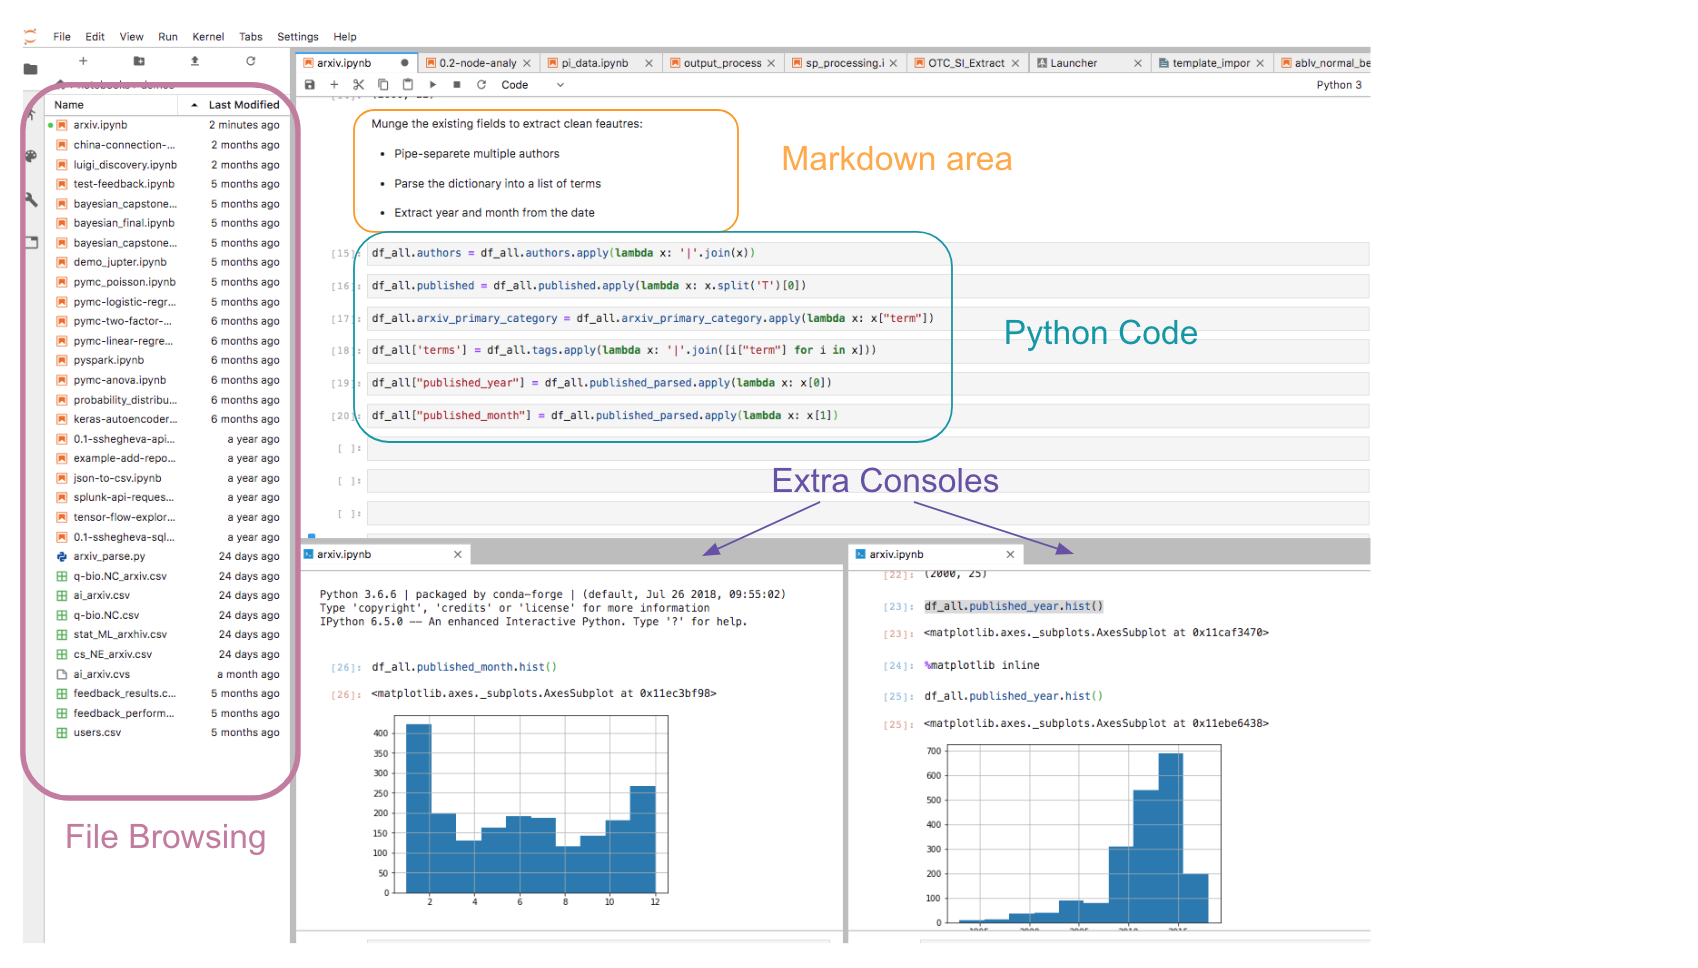
\includegraphics[scale=.5]{figures/project-principles/jupyter.png}
\caption{An example of JupyterLab Workspace.}
\label{fig::1}
\end{figure}

\subsubsection*{What works well}

\textbf{The Gulfs of Execution and Evaluation}

The most attractive feature of the Jupyter environment - \textbf{interactivity} - thrives in both \textit{gulfs}: \textit{execution} and \textit{evaluation}. The execution gulf is easily bridged as the cells provide a clear indication for where text/code should be entered. In the early stage of \textit{planning} where the user has to choose an appropriate action out of all possible actions, the interface positions a blinking cursor at the beginning of a cell thus prompting the user to enter a code inside it. This follows the \textit{consistency} principle for designing interfaces where the user can easily transfer the learning across different systems (think, any modern text editors). 

Similarly to other IDEs, the interface provides functionality for syntax highlighting that enables an easier code interpretation. Being able to quickly \textit{read} the code narrows the \textit{gulf of evaluation} by fostering a better understanding of the code blocks. The Project Jupyter currently supports several dozens of languages, so the user does not have to jump between different IDEs to create their code in a more natural environment than the basic text editors. 

Unlike other code editors, Jupyter Notebooks signals the state of each cell by 1) assigning it a number in the brackets at the beginning of the cell if it has been executed; 2) leaving it empty if it has not been run; 3) using asterisk to show that a cell is \textit{in progress}. At the \textit{perceiving} stage of what happened, the gulf of evaluation is bridged and provides a good \textit{mileage} towards task execution. 

\textbf{Direct Manipulation}

Cells are viewed as physical building blocks, and as such can be re-arranged using a \textit{direct manipulation} via \textbf{drag-n-drop} functionality \cite{frohlich1997direct}. The user is engaged in the process of completing their task by 1) planning the action by hovering over the cell that needs to be moved; 2) grabbing the cell and dragging it over the area that specifies the new location; 3) releasing the hold when the cell is aligned with the desired destination. For the described task, the interface becomes \textit{invisible} and intuitive largely due to the tight relationships between the two gulfs. As the user is working on their task of cell re-arrangement, the system provides a "hint" in the form of target line for where the new cell would land before the action is complete \footnote{It is challenging to capture the drag-and-drop action with a screenshot.}. The \textit{feedback} is easy to interpret, and it matches with what the user is expecting to happen. Therefore, the goal can be accomplished more accurately (cell is in the correct position) and more efficiently (speed of execution) without the user focusing on the interface.

\textbf{Feedback}

The Jupyter interface is highly interactive. Compared to other more traditional IDEs (Integrated Development Environment), the Jupyter Lab has a much narrower \textit{gulf of evaluation}. The action of \textit{Running} a cell yields immediate feedback that allows the user assessing how well their intentions have been met. The output is displayed \textit{asynchronously} as it is generated in the Kernel allowing user to \textit{perceive}, \textit{interpret}, and \textit{compare} the state of the execution with their goal or a sub-goal. 

This format drives more direct exploration as the user can see what happens after each step. The interface enables rapid iterations that enhances the usability. Instead of re-running an entire module, each cell can be executed individually that may save significant time in troubleshooting code. 

\subsubsection*{What doesn't works well}

\textbf{Ease and Comfort Principle}

Drag-n-dropping cells work pretty well when the distance between the positions (current and the desired) is small. As the distance increases, and the user has to scroll through the page while simultaneously "dragging" a cell, the \textbf{ease, and comfort} principles are infringed that reduce the overall efficiency in accomplishing the task \cite{story1998universal}. If the distance between the current and the target location spans across a few pages, then the user has to perform a few "stops" by splitting their action of \textit{move} into a sequence of drag-n-drops and page scrolls. 

\textbf{Slips in the Gulf of Execution} 

Current implementation of the interface provides signifiers located in the toolbar for \textbf{adding} (plus sign) and \textbf{deleting} (scissors icon) cells (see Figure~\ref{fig::2}). 

\begin{figure}[hbt!]
\centering
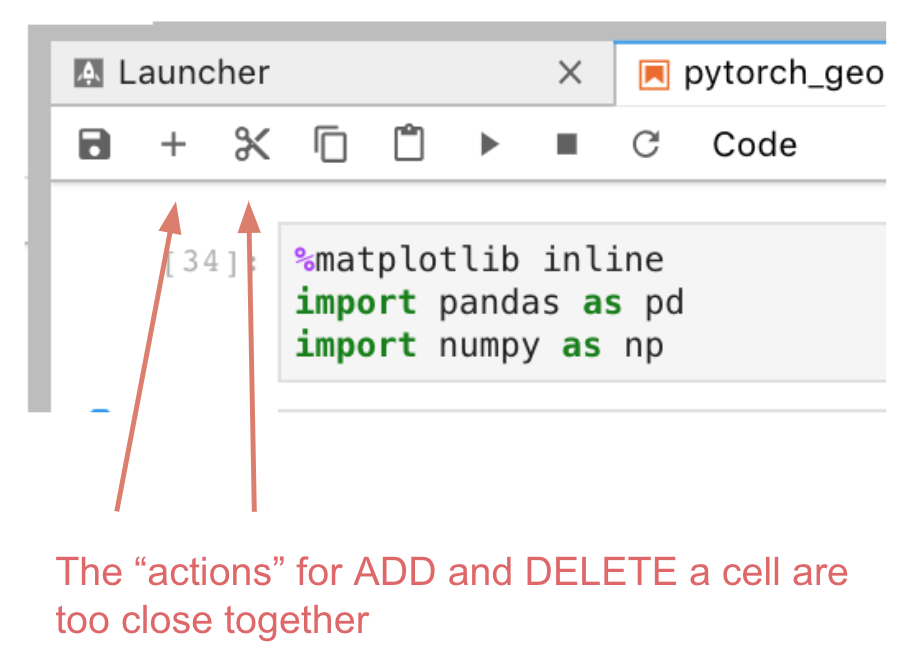
\includegraphics[scale=.4]{figures/project-principles/jupyter_add_delete.png}
\caption{Aspect of the interface that allow Slip errors}
\label{fig::2}
\end{figure}

There are two issues with the chosen position for those two opposing operations: 

1) by placing them \textit{next to each other}, the interface invites user errors such as \textit{slips}; the user accidentally clicks on \textit{delete} instead of the intended \textit{add} action. \footnote{I have personally made this type of slip numerous times wishing the interface was less inviting for accidental actions}  

2) by situating them on the toolbar, the \textit{gulf of execution} is widened at the stage of \textit{performing} an action; the user has to move the mouse from the current location to the toolbar to perform either of these most frequent actions.

The user has a correct \textbf{mental model} on how to add or delete a cell as the icons for signifiers are self-explanatory and consistent. However, a user intending to do one action, such as cell addition, may inadvertently execute the opposing one - deletion. This is an example of \textit{action-based} slip that occurred due to a rushed user behavior \cite{norman2013design}.

A sub-optimal interaction with executing the action (add/delete) presents itself again when the notebook is large enough that the user needs to move the mouse between the current position and the toolbar. This increases the \textbf{gulf of execution} and decreases the efficiency especially for new users who have not learned the shortcuts for these commands.  


\textbf{Discoverability}

Another feature that contributes to a wide execution gulf is \textbf{merging} cells that is a commonly requested action. The aspect of the interface that is designated for this functionality violates the \textit{discoverability} principle. Unlike other operations, merging is only accessible via \textit{Edit} Menu -> Merge Selected Cells and thus not immediately visible or easily discoverable \cite{jayasimman2011dynamic}. The contextual menu available at the right-click of the mouse button does not include the pointer to the merging operation. The mismatch between menus fails the consistency check \textit{within} the application, and further increases the \textit{gulf of execution}.  Figure~\ref{fig::3} shows the \textit{merging} operation accessible in the \textit{Edit} menu, beyond which there is no indication that an operation is possible at all.

\begin{figure}[hbt!]
\centering
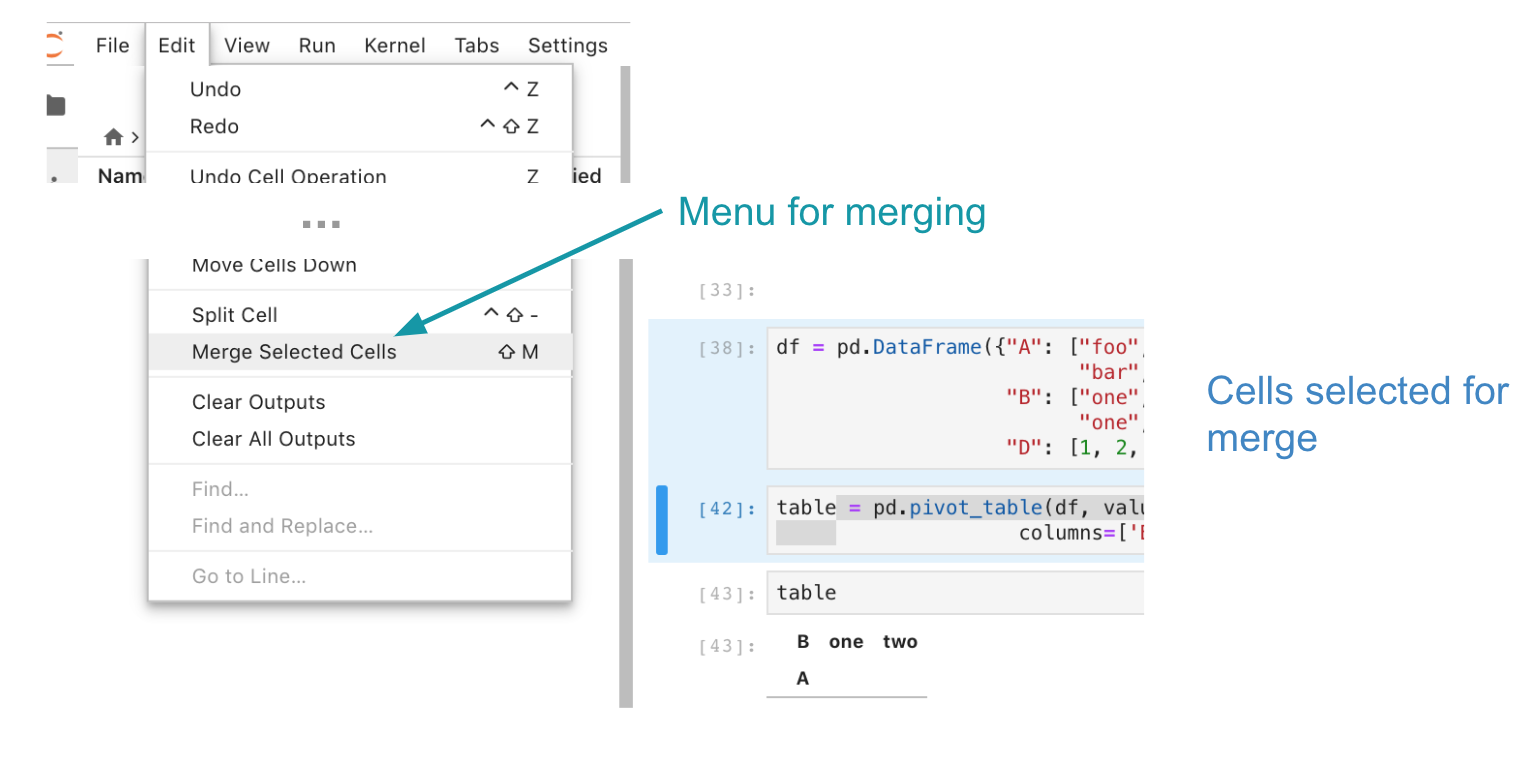
\includegraphics[scale=.4]{figures/project-principles/cell_merge_eval.png}
\caption{Limited visibility for cell merging functionality.}
\label{fig::3}
\end{figure}


\subsection*{Interface Redesign}
Based on the evaluation performed above, we redesign the \textit{Notebook} section by adding \textbf{six} different components that can improve the interactions between the user and the interface.

\begin{figure}[hbt!]
\centering
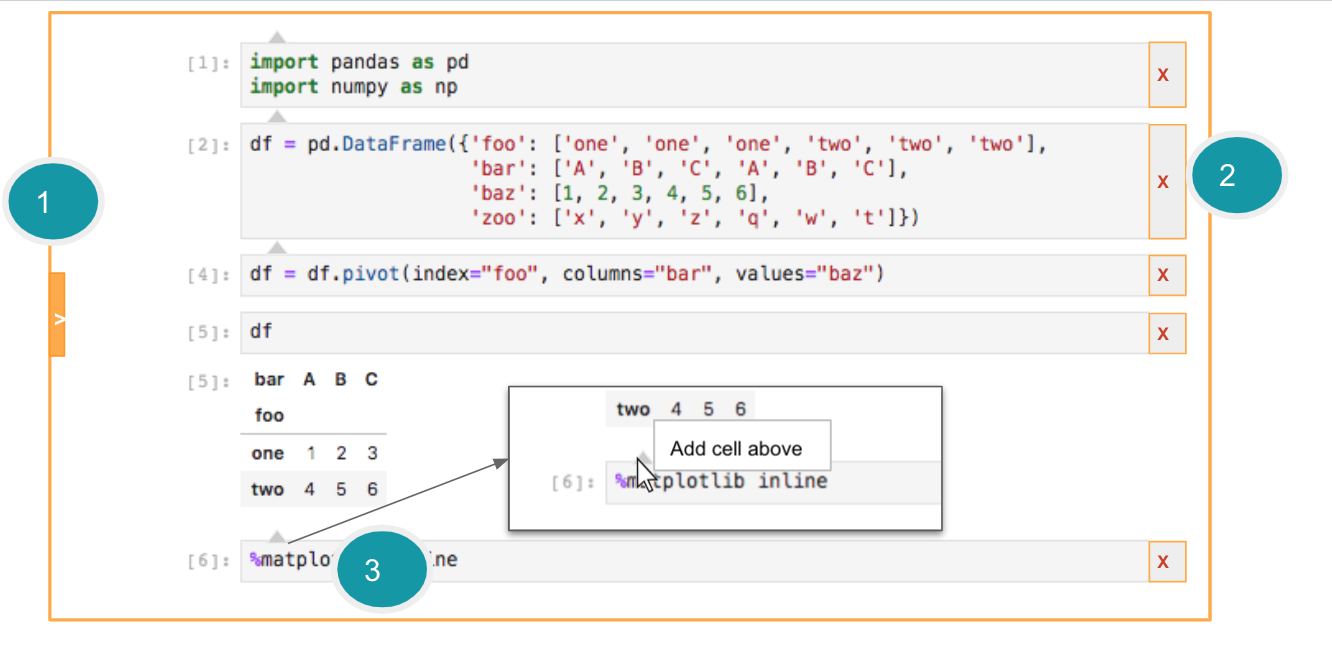
\includegraphics[scale=.5]{figures/project-principles/jupyter_mock_screen_a.png}
\caption{Screen A: Mockup of the Jupyter Notebook Interface. The first three components: 1) Sidebar expansion 2) Affordance for cell additions 3) Affordance for cell deletions}
\label{fig::4}
\end{figure}

\subsubsection*{1. Expand/Collapse Side Bar}
Figure~\ref{fig::4} (in the area labeled as 1) shows a small arrow in the left side (mid-point) that suggests that an area has been \textit{collapsed} and it can be \textit{expanded}. The expansion area is designed to reveal \textbf{newly-designed} controllers and hide them when not needed \footnote{This feature is inspired by the recent Overleaf redesign}. After the expansion, the sidebar (see Figure~\ref{fig::5}) displays the additional affordances described below.

\subsubsection*{2. Delete a Cell / Undo the Delete}
The rightmost edge of the cell is augmented with a \textit{right cross}  that suggest that a cell can be deleted by clicking on the little rectangle area (see Figure~\ref{fig::undo}). When the user clicks on the red cross, the icon changes to a \textit{circled arrow} pointing anti-clockwise that signifies that an \textit{undo} operation is available. The cell becomes greyed-out for a few seconds until it disappears entirely.

\begin{figure}[hbt!]
\centering
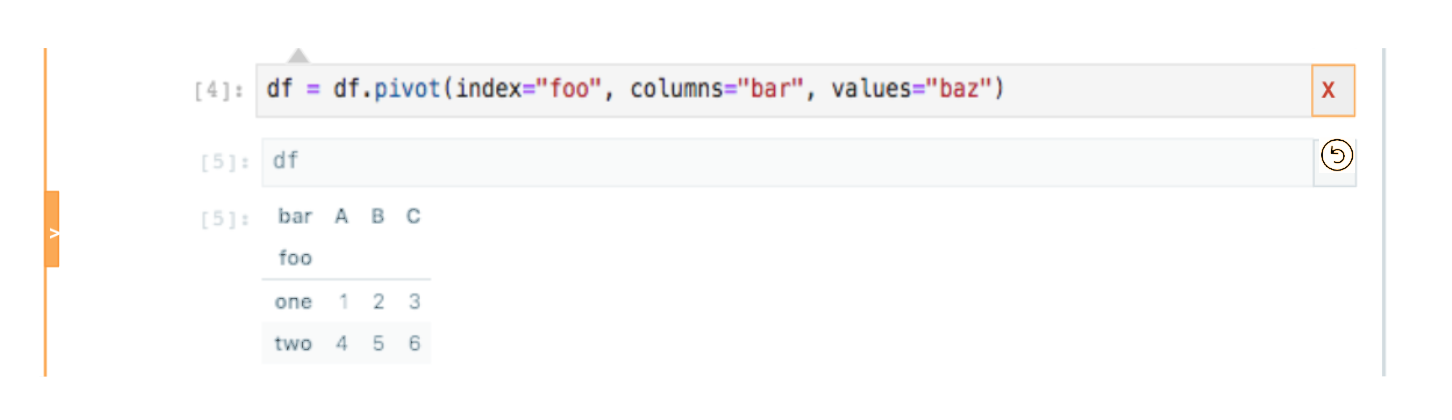
\includegraphics[scale=.5]{figures/project-principles/delete_undo.png}
\caption{Delete/Undo Operation via Affordance of Red Cross and Circled Arrow pointing anti-clockwise. The deleted cell is greyed-out for a short period of time before dissapearing.}
\label{fig::undo}
\end{figure}

\subsubsection*{3. Ticker to Add Cells}
In the redesign, each cell decorated with a small tick in the shape of a \textit{triangle} that upon hovering over with a mouse will give a \textit{hint} for the action. By clicking on the triangle, a new cell line is added above (see Figure~\ref{fig::4} - section labeled as 3)

\begin{figure}[hbt!]
\centering
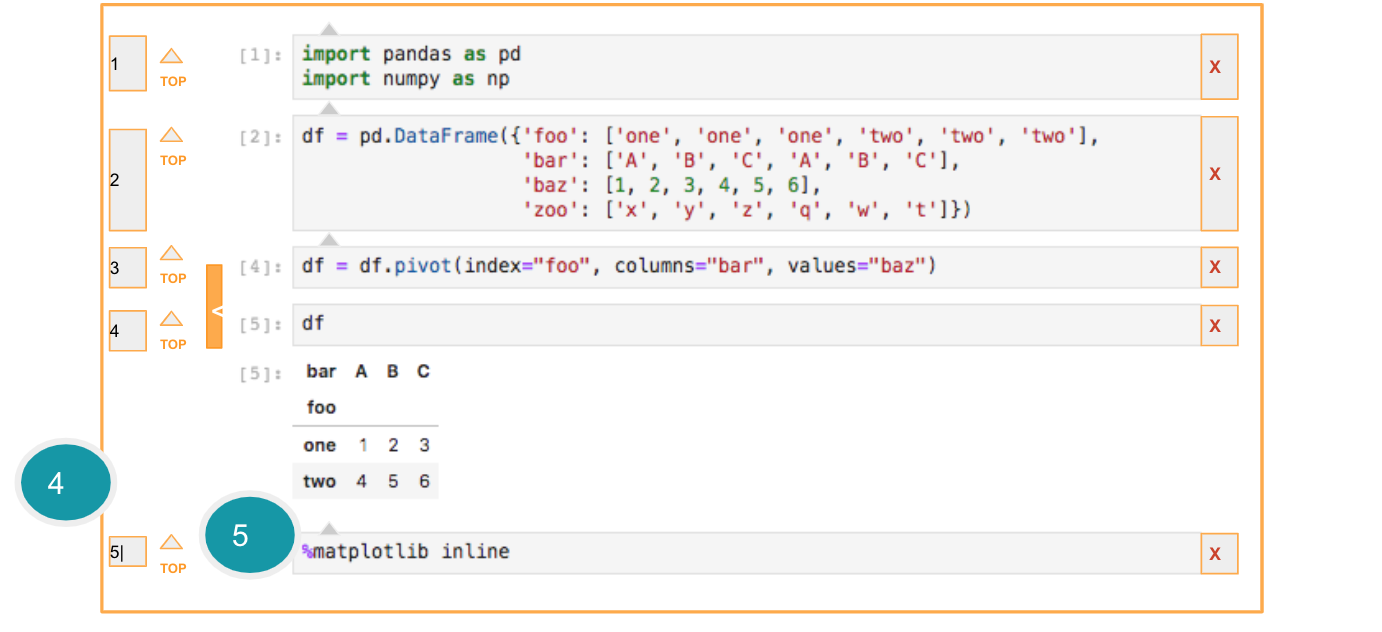
\includegraphics[scale=.5]{figures/project-principles/jupyter_mock_screen_b.png}
\caption{Screen B: Mockup of the Jupyter Notebook Interface. The additional two components 4) Re-order the cells 5) Move a cell to the top position.}
\label{fig::5}
\end{figure}

\subsubsection*{4. Force order the cells}
Figure~\ref{fig::5} demonstrates the features that become available after the sidebar has been extended. Here we have a depiction of each cell where a user can enter a number to force the order of the cells (see the section labeled as 4). This feature is inspired by Netflix's movie queue. 

\subsubsection*{5. Move to the top}
Another feature inspired by the Netflix's queue management is an \textit{arrow} and \textit{top} that allow the user to move certain cells to the top of the queue (most applicable to \textit{import} cells). Both features (force order and move to the top) are hidden from the default view to avoid the clutter.


\subsubsection*{6. In-context Operations}
The last feature in the redesign is shown in Figure~\ref{fig::6}, and it appear upon \textit{cell-selection} operation. 

\begin{figure}[hbt!]
\centering
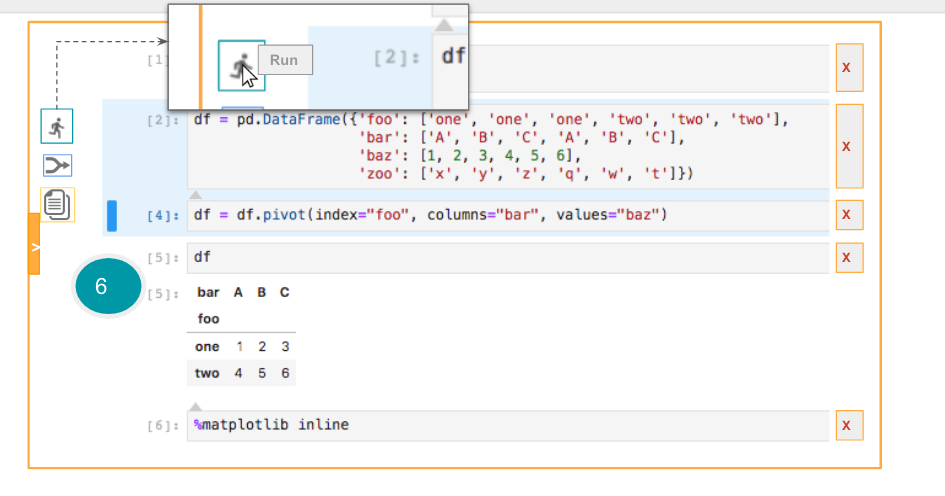
\includegraphics[scale=.35]{figures/project-principles/jupyter_mock_screen_c.png}
\caption{Screen C: Mockup of the Jupyter Notebook Interface. The last component: 6) Expose contextual controls upon cell selection.}
\label{fig::6}
\end{figure}

In the mock-up screen, when the user highlights a sequence of cells, the interface suggests three possible operations:

\begin{itemize}
\itemsep0em 
    \item \textit{Run} the selected cells depicted by an icon of a running person
    \item \textit{Merge} the selected cells depicted by an icon of arrow connected at a point.
    \item \textit{Copy} the selected cells depicted by an icon of two stacked papers.
\end{itemize}

Although the described operations are represented by visual icons, when the user places their mouse over designated areas, an additional small pop-up area appears with \textit{text} labels for the functions - \textit{Run}, \textit{Merge}, \textit{Copy}. Figure~\ref{fig::6} includes the \textit{zoomed-in} screen section to show the example of \textit{hover-over} text for a \textit{Run} controller.



\subsection*{Interface Justification}
All six features enable a more efficient access to the operations over cells, such as \textit{addition}, \textit{deletion}, \textit{reorder}, \textit{merge}, \textit{copy}, and \textit{run}.

\textbf{Discoverability}

The main principle driving redesign in the presented interface is improving the \textit{discoverability}. Larry Constantine and Lucy Lockwood advocated for a design the makes options needs for a task \textit{visible} without extraneous efforts from the user \cite{jayasimman2011dynamic}. The previously hidden operation for \textit{merging} cells now appears as an icon among two other most common operations - \textit{run} and \textit{copy}. In addition to providing easy access to those actions, their functionality is further identified by \textit{callouts} than appear upon mouse hover-overs. This enables the user, especially a novice, to explore the interface and learn its capabilities. 

The new affordances for operations of \textit{add} and \textit{delete} are similarly provisioned with callout menus that give users additional clues for possible interactions with the interface. The discoverability is improved by presenting a redesign that applies the fundamental concepts, such as \textit{affordances}, \textit{signifiers} and \textit{mappings}, to uncover a functionality that can positively impact the user's experience. 

\textbf{The Gulf of Execution}

In addition to enhancing the discoverability, the same affordances and signifiers, narrow down the \textit{gulf of execution}, specifically at the stages of \textit{planning} and \textit{performing}. By allowing the user to \textit{delete} a cell by clicking on the red cross shown for \textit{each} cell, the action can be executed faster than navigating to the toolbar for clicking the \textit{scissors} icon. The planning portion is simplified by removing the confusion for which cell is intended to be deleted. 

A user who seeks to insert a new cell is relieved from having to reach to the toolbar for the \textit{plus} sign each time the action is needed. By introducing a small tick above each cell, the user can unequivocally insert a cell in the desired place. Inevitably, this further contributes to the \textit{directness} of the interface described earlier on an example of drag-n-drop functionality. 

The new contextual toolbar, consisting of three operations - \textit{run}, \textit{merge} and \textit{copy} brings the user closer the action. The menu appears upon an \textit{event} of cell(s) selection, so it does not impede the workflow of adding and executing new cells. Evaluating the gulf of execution gave clues for the areas that could benefit from a redesign to enhance the interaction. 

\textbf{Proximity Constraints}

The evaluation section described an area in the interface where users can make a \textit{slip} in a rush. This type of error can be minimized by forcing some type of constraints. The redesign exercises this principle by \textit{separating} in space the affordances for \textit{addition} and \textit{deletion}. Previously, the buttons were located next to each other allowing for a possibility to choose the wrong action. The redesign addresses that by placing an affordance for adding a cell on the leftmost edge, and affordance for deletion on the rightmost edge, thus imposing a \textit{proximal constraint}.  Additionally, the action for the actual icon for deletion is made more prominent by changing its color to red. This ensures that even when distracted or in a rush, the user is more likely to choose a correct action.

\textbf{Flexibility}

Designing for everyone means that interface may need to include accelerators that can speed up some of the interactions \cite{nielsen1994usability}. In the redesigned version of the interface, a user can expand the sidebar (the expansion is afforded by the arrow) to access additional functionality related to \textit{cell ordering}. When a user wants to move a cell up without dragging it, or copy/pasting it, a new action is afforded by assigning a cell a new number (higher or lower). Similarly to how Netflix interface manages users' movie queue by allowing them the re-arrange the order of titles, the cells in Notebooks can be moved to predefined positions. 

One of the criticisms for the Notebooks interface is the fact that it encourages the poor coding practice by allowing the cells to be executed out of order \cite{perkel2018jupyter}. And, while the new redesign, does enforce a different user behavior, it makes it easier to organize the cells that can follow a more logical flow. Additionally by making the \textit{merging} functionality more accessible (in the event of cell selection), the user can combine cells into units that can be refactored into reusable functions. 

Thus, the interface preserves it's widely embraced interactivity that \textit{gives great power for exploration} \footnote{a quote from Lorena Barba, a  mechanical and aeronautical engineer at George Washington University in Washington DC} while also providing means to structure and organize the code.


\textbf{Cognitive Load}

In designing good interfaces, it is imperative to strike a balance between the \textit{discoverability} via visible operations and \textit{simplicity} via minimalism. In the redesign, this is achieved by adding an affordance to \textit{collapse} the sidebar with the extended functionality when not used. This follows the principle of \textit{reducing the clutter} to avoid unnecessary user distractions. Hiding the sidebar lessens the cognitive load on the user interacting with the interface. 

Another aspect of the redesign that addresses the principle of cognitive load is enabling the \textit{callout} menus when the user hovers over a visual icon. In some instances, for example, representing the \textit{run} function with a picture of a \textit{running man} communicated the operation efficiently. In other instance, the icon may not have that power as the user cannot easily associate the action with the icon image. In such cases, it is imperative to provide the user with additional clues in the form of pop-up text describing the activity. Thus, instead of having them remember the action or \textit{figure it out}, the user can be reminded of it when needed.  

\textbf{Feedback and Tolerance}

The outcome of the action to add a cell is a new empty cell. The result of the deletion of the cell is that it disappears immediately. If a cell was deleted unintentionally, in the current interface the user can to reach out the main menu and find an \textit{undo} operation. 

The redesign adds a slight delay between execution of the delete operation and removing the cell from the notebook. In the window of a few seconds, the deleted cell is \textit{greyed-out} to communicate the outcome \textit{before} it disappears from the screen. Furthermore, the red-cross is replaced with an arrow pointing anti-clockwise to give the user a more convenient way to reverse the operation. This feature applies a \textit{tolerance} principle to provide the user with a chance to rethink the executed transaction. If the action was performed due a slip, a small delay window should be sufficient to correct the action.

\bigbreak
In \textbf{conclusion}, the new interface fully preserves the positive elements while enhancing the user's experience in navigating the capabilities of the interface. Most of the added functionality does not impact the advanced users who are accustomed to numerous keyboard short-cuts while performing the frequent operations. Novices, on the other hand, would benefit greatly from a more user-friendly interactions. Future redesigns may target the expert users by providing means to customize their layouts. 

\bibliographystyle{apacite} 
\bibliography{bibtemp}

\end{document}
